\documentclass{article}
\usepackage[utf8]{inputenc}
\usepackage{amsmath, amssymb,amsfonts}
\usepackage{graphicx}
\usepackage{geometry}
\usepackage{booktabs}
\usepackage{caption}
\usepackage{longtable}
\usepackage{array}

\geometry{a4paper, margin=1in}

\title{Support Vector Machine Analysis and Optimization on the Glass Identification Dataset}
\author{Eduardo Henrique Basilio de Carvalho}
\date{May 27, 2025}

\begin{document}

\maketitle

\begin{abstract}
This report details the application and optimization of a Support Vector Machine (SVM) classifier on the Glass Identification dataset. The study involves data preprocessing, initial model evaluation, and two distinct hyperparameter optimization strategies. The first optimization focuses on maximizing classification certainty and inter-class probability spread. The second optimization utilizes a custom metric, the Segment Attractiveness and Homogeneity (SAH) score, to guide hyperparameter selection. Model performance is primarily assessed using accuracy, and likelihood space visualizations provide qualitative insights into the classifier's behavior.
\end{abstract}

\section{Introduction}
The Glass Identification dataset was used to train and evaluate an SVM classifier. The primary goal was to distinguish between a majority class and all other classes, effectively creating a binary classification problem. This report outlines the preprocessing steps, the SVM pipeline construction, initial performance evaluation, and subsequent hyperparameter tuning using two different objective functions.

\section{Data Preprocessing and Initial Pipeline}
The Glass Identification dataset was loaded using the `ucimlrepo` library. The target variable $y$ was binarized by identifying the majority class and labeling it as class 0, while all other instances were labeled as class 1.

A machine learning pipeline was constructed with the following steps:
\begin{enumerate}
    \item \textbf{StandardScaler}: Standardizes features by removing the mean and scaling to unit variance.
    \item \textbf{VarianceThreshold(threshold=0.1)}: Removes features with variance below 0.1.
    \item \textbf{CorrelationFilter(threshold=0.9)}: Removes features that have a Pearson correlation coefficient greater than 0.9 with a feature of a lower index. The correlation matrix $\mathbf{R}$ is computed for the $n_f$ features. For an upper triangular mask $\mathbf{U}$ (excluding the diagonal), features $j$ are marked for removal if $|\mathbf{R}_{ij}| > 0.9$ for any $i < j$ where $\mathbf{U}_{ij}$ is true.
    \item \textbf{SVC(probability=True)}: A Support Vector Classifier with probability estimation enabled. Default parameters are used initially.
\end{enumerate}

Cross-validation was performed using a `StratifiedKFold` strategy with 10 splits and shuffling enabled.

\section{Initial Model Evaluation}
The SVM pipeline was evaluated using 10-fold stratified cross-validation. The performance results were:
\begin{itemize}
    \item Individual fold accuracies: ['0.77', '0.68', '0.86', '0.64', '0.76', '0.81', '0.86', '0.86', '0.62', '0.76'] 
    \item Mean Accuracy: $0.76 \pm 0.09$ 
    \item Accuracy Range: $0.62 - 0.86$ 
\end{itemize}

The model was then trained on the full dataset, and the predicted probabilities $Q = P(\text{class } i | X)$ were obtained. $Q_0$ represents $P(\text{class } 0 | X)$ and $Q_1$ represents $P(\text{class } 1 | X)$. Figure \ref{fig:likelihood_initial} shows the likelihood space plot for the initial model.

\begin{figure}[htbp]
    \centering
    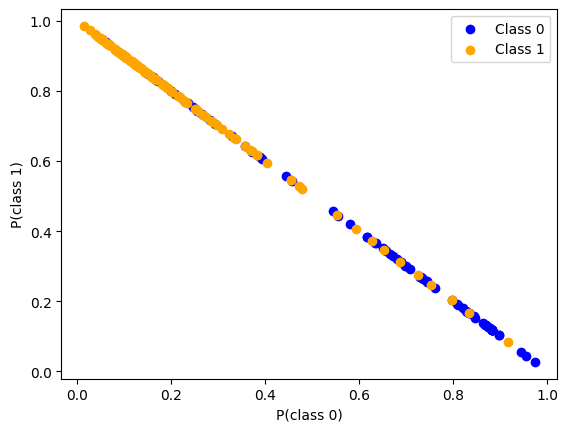
\includegraphics[width=0.7\textwidth]{figure_1.png}
    \caption{Likelihood space plot for the initial SVM model. $P(\text{class 0})$ vs $P(\text{class 1})$ for each sample, colored by true class label.}
    \label{fig:likelihood_initial}
\end{figure}

\subsection{Certainty and Spread Metrics}
To further evaluate the model's probability predictions, two metrics were defined:
\begin{itemize}
    \item \textbf{Certainty for Class 0 ($C_{C0}$)}: The mean absolute distance of predicted $P(\text{class } 0)$ values from 1.0, for samples actually belonging to class 0. Let $Q_{0C0}$ be the set of $P(\text{class } 0)$ predictions for true class 0 samples.
    $$ C_{C0} = \text{mean}(|Q_{0C0} - 1.0|) $$ 
    \item \textbf{Certainty for Class 1 ($C_{C1}$)}: 1.0 minus the mean absolute distance of predicted $P(\text{class } 0)$ values from 1.0, for samples actually belonging to class 1. Let $Q_{0C1}$ be the set of $P(\text{class } 0)$ predictions for true class 1 samples.
    $$ C_{C1} = 1.0 - \text{mean}(|Q_{0C1} - 1.0|) $$ 
    \item \textbf{Spread for Class 0 ($S_{C0}$)}: The mean absolute difference between all pairs of $P(\text{class } 0)$ predictions for samples within class 0.
    $$ S_{C0} = \text{mean}(|Q_{0C0,i} - Q_{0C0,j}|) \quad \forall i \neq j $$ 
    \item \textbf{Spread for Class 1 ($S_{C1}$)}: The mean absolute difference between all pairs of $P(\text{class } 0)$ predictions for samples within class 1.
    $$ S_{C1} = \text{mean}(|Q_{0C1,i} - Q_{0C1,j}|) \quad \forall i \neq j $$ 
\end{itemize}
For the initial model, these metrics were:
\begin{itemize}
    \item Certainty for Class 0: $0.37$ 
    \item Certainty for Class 1: $0.21$ 
    \item Spread for Class 0: $0.29$ 
    \item Spread for Class 1: $0.17$ 
\end{itemize}

\section{Hyperparameter Optimization based on Certainty and Spread}
The SVM hyperparameters $C$ and $\gamma$ were optimized using \texttt{dual annealing}. The objective function aimed to maximize the mean certainty and mean spread, while penalizing imbalances between the certainties and spreads of the two classes.
Let $\bar{C} = (C_{C0} + C_{C1})/2$ and $\bar{S} = (S_{C0} + S_{C1})/2$.
Let $\Delta C = |C_{C0} - C_{C1}|$ and $\Delta S = |S_{C0} - S_{C1}|$.
The score to be maximized was $ \text{Score} = \bar{C} + \bar{S} - \Delta C - \Delta S $. The optimizer minimizes the negative of this score.
The bounds for $C$ and $\gamma$ were set to $[0.1, 5]$.

The optimization yielded:
\begin{itemize}
    \item Best $C$: $0.3415$ 
    \item Best $\gamma$: $0.1032$ 
\end{itemize}

The metrics for the model retrained with these optimal parameters were:
\begin{itemize}
    \item Optimized Certainty for Class 0: $0.38$ 
    \item Optimized Certainty for Class 1: $0.26$ 
    \item Optimized Spread for Class 0: $0.26$ 
    \item Optimized Spread for Class 1: $0.19$ 
\end{itemize}

Cross-validated results with these optimized parameters were:
\begin{itemize}
    \item Individual fold accuracies: ['0.64', '0.64', '0.64', '0.64', '0.76', '0.76', '0.71', '0.67', '0.71', '0.67'] 
    \item Mean Accuracy: $0.68 \pm 0.05$ 
    \item Accuracy Range: $0.64 - 0.76$ 
\end{itemize}

Figure \ref{fig:likelihood_optimized_certainty_spread} shows the likelihood space for this optimized model.

\begin{figure}[htbp]
    \centering
    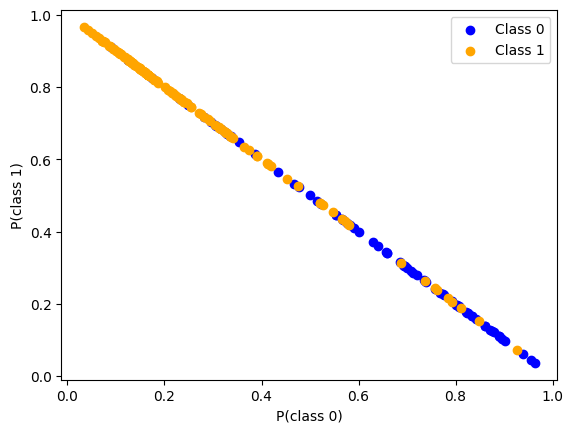
\includegraphics[width=0.7\textwidth]{figure_2.png}
    \caption{Likelihood space plot for the SVM model optimized using certainty and spread metrics.}
    \label{fig:likelihood_optimized_certainty_spread}
\end{figure}

\section{Segment Attractiveness and Homogeneity (SAH) Score}
The SAH score is a metric ranging from 0 to 1, designed to quantify how well points are homogeneously spread within a defined segment $[a, b]$. An SAH score of 1 represents an ideal distribution.

\subsection{SAH Calculation}
Given a 1D array of points $P = \{p_1, p_2, ..., p_n\}$, and segment boundaries $a, b$ (with $a < b$). The segment length is $L = b - a$.

\begin{enumerate}
    \item \textbf{Segment Attractiveness Weight Function $w(p_i)$}:
    For each point $p_i$, its distance $d_S(p_i)$ from the segment $[a,b]$ is calculated:
    $$ d_S(p_i) = \begin{cases} a - p_i & \text{if } p_i < a \\ 0 & \text{if } a \le p_i \le b \\ p_i - b & \text{if } p_i > b \end{cases} $$
    The weight $w(p_i)$ is then given by:
    $$ w(p_i) = \exp\left(\frac{-2 \cdot d_S(p_i)^2}{L^2}\right) $$

    \item \textbf{Mean Attractiveness (MA)}:
    If $n=0$, $MA=0.0$. Otherwise:
    $$ MA = \frac{1}{n} \sum_{i=1}^{n} w(p_i) $$

    \item \textbf{Weighted Homogeneity ($H_W$)}:
    $H_W = 1.0$ if $n \le 1$. Otherwise, points are sorted $P_{sorted}$, and corresponding weights are $W_{sorted}$.
    Let $W_{sum} = \sum w_i$. If $W_{sum} \approx 0$, $H_W = 1.0$.
    Nearest neighbor distances $d_{nn,i}$ are calculated for sorted points.
    \begin{itemize}
        \item Weighted mean of nearest neighbor distances ($\mu_d$):
        $$ \mu_d = \frac{\sum (d_{nn,i} \cdot w_{sorted,i})}{W_{sum}} $$
        \item Weighted variance of nearest neighbor distances ($\sigma_d^2$):
        $$ \sigma_d^2 = \frac{\sum ((d_{nn,i} - \mu_d)^2 \cdot w_{sorted,i})}{W_{sum}} $$
        \item Weighted coefficient of variation ($CV_d$):
        If $\mu_d \approx 0$, $CV_d = 0.0$. Otherwise:
        $$ CV_d = \frac{\sqrt{\sigma_d^2}}{\mu_d} $$
    \end{itemize}
    The homogeneity score $H_W$ is:
    $$ H_W = \frac{1.0}{1.0 + CV_d} $$

    \item \textbf{Final SAH Score}:
    $$ \text{SAH} = MA \times H_W $$
\end{enumerate}

For the initial SVM model (default parameters), the SAH scores were calculated for $Q_0$ predictions:
\begin{itemize}
    \item SAH Score for Class 0 ($Q_{0C0}$, segment $[0.5, 1.0]$): $0.4260$ 
    \item SAH Score for Class 1 ($Q_{0C1}$, segment $[0.0, 0.5]$): $0.2951$ 
\end{itemize}

\section{Hyperparameter Optimization based on SAH Score}
The SVM hyperparameters $C$ and $\gamma$ were optimized again using \texttt{dual annealing}, this time with an objective function based on SAH scores.
Let $SAH_0$ be the SAH score for class 0 probabilities ($Q_{0C0}$) within the segment $[0.5, 1.0]$, and $SAH_1$ be the SAH score for class 1 probabilities ($Q_{0C1}$) within the segment $[0.0, 0.5]$.
The objective was to maximize $\text{mean}(SAH_0, SAH_1) - |SAH_0 - SAH_1|$. The optimizer minimizes the negative of this score.
The bounds for $C$ and $\gamma$ were $[0.1, 5]$.

The SAH optimization yielded:
\begin{itemize}
    \item Best $C$ (sah\_C): $0.4686$ 
    \item Best $\gamma$ (sah\_gamma): $0.1770$ 
\end{itemize}

After retraining with these SAH-optimized parameters, the SAH scores were:
\begin{itemize}
    \item Optimized SAH Score for Class 0: $0.3887$ (Note: page 11 reports 0.3847 initially, then page 12 output reports 0.3887 after final run with sah\_C, sah\_gamma) 
    \item Optimized SAH Score for Class 1: $0.3443$ (Note: page 11 reports 0.3461 initially, then page 12 output reports 0.3443 after final run) 
    \item Difference: $0.0443$ 
\end{itemize}

Cross-validated results with SAH-optimized parameters were:
\begin{itemize}
    \item Individual fold accuracies: ['0.77', '0.73', '0.59', '0.73', '0.81', '0.86', '0.86', '0.76', '0.81', '0.76'] 
    \item Mean Accuracy: $0.77 \pm 0.07$ 
    \item Accuracy Range: $0.59 - 0.86$ 
\end{itemize}

Figure \ref{fig:likelihood_optimized_sah} shows the likelihood space for the SAH-optimized model.

\begin{figure}[htbp]
    \centering
    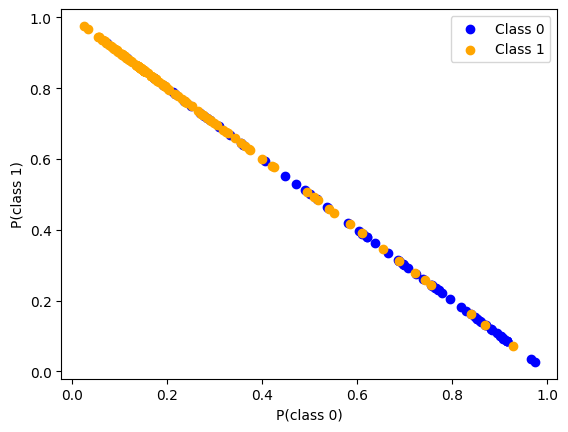
\includegraphics[width=0.7\textwidth]{figure_3.png}
    \caption{Likelihood space plot for the SVM model optimized using SAH score.}
    \label{fig:likelihood_optimized_sah}
\end{figure}

\section{Summary of Results}
The study explored different approaches to SVM classification and hyperparameter tuning. The table below summarizes the mean cross-validated accuracies:

\begin{table}[htbp]
\centering
\caption{Comparison of Mean Accuracies for Different SVM Models.}
\begin{tabular}{lcc}
\toprule
Model Configuration & Mean Accuracy & Std. Dev. \\
\midrule
Initial SVM (Default Parameters) & $0.76$  & $0.09$  \\
Optimized (Certainty \& Spread) & $0.68$  & $0.05$  \\
Optimized (SAH Score) & $0.77$  & $0.07$  \\
\bottomrule
\end{tabular}
\label{tab:accuracy_summary}
\end{table}

The initial SVM model provided a mean accuracy of $0.76$. Optimization based on certainty and spread metrics led to a decrease in mean accuracy to $0.68$, although it aimed to improve the quality and balance of probability distributions. The optimization based on the SAH score slightly improved the mean accuracy to $0.77$ compared to the initial model, and also aimed for better distributional properties within defined probability segments. The SAH-optimized model also achieved a balanced SAH score between the two classes (0.3887 for Class 0 vs 0.3443 for Class 1).

\end{document}
